\chapter{PHƯƠNG PHÁP TIẾP CẬN}

\section{Phân tích ba kỹ thuật tiêu biểu}

Nhóm chọn ba phương pháp (Hình 3.1) vì: (i) Bảng II \cite{ref1} lấy \textbf{DIN-SQL} \cite{ref4} đại diện C1, \textbf{DAIL-SQL} \cite{ref5} đại diện C2; \textbf{MAC-SQL} \cite{ref6} là ví dụ \emph{multi-agent} ở Mục IV-A2, IV-A5; (ii) DAIL-SQL, MAC-SQL có cả bản FT (Bảng IV); (iii) cả ba là dẫn chứng của \cite{ref1} ở Mục V-VI và có mã nguồn công khai.

\subsection{Kỹ thuật DIN-SQL}

\textbf{DIN-SQL} \cite{ref4} thuộc \textbf{C1 - Decomposition} và \textbf{C4 - Execution Refinement}, dùng GPT-4\textasteriskcentered{} (Bảng III \cite{ref1}). Ý tưởng chính là chia bài toán thành \emph{pipeline} bốn giai đoạn (Mục IV-A2): (1) \textbf{Schema Linking}, tuần tự hóa \emph{schema} thành \emph{prompt} ngôn ngữ tự nhiên kèm \emph{foreign-key hints} (Mục V-A2); (2) \textbf{Classification}; (3) \textbf{SQL Generation}; (4) \textbf{Self-Correction}, dùng \emph{generic or gentle prompts} để LLM nhận ra \emph{schema misalignments} rồi sinh lại SQL (Mục IV-A5). \emph{Question decomposition} chỉ phụ trợ, trọng tâm là \emph{module-level collaboration}. Hạn chế nhóm tác giả nêu: \emph{pipeline} nhiều giai đoạn làm tăng lượt gọi API và chi phí (Mục VI-B).

\subsection{Kỹ thuật DAIL-SQL}

\textbf{DAIL-SQL} \cite{ref5} thuộc \textbf{C2 - Prompt Optimization} và \textbf{C3 - Reasoning Enhancement} (Bảng III), đồng thời thuộc \textbf{FT - Data Augmentation} (Bảng IV) \cite{ref1}. Ý tưởng chính là nâng chất lượng \emph{prompt}. Với \emph{zero-shot} (Mục IV-A1), DAIL-SQL đánh giá năm kiểu \emph{prompt} tổ hợp từ \emph{instruction}, \emph{rule implication}, \emph{foreign key}, kèm quy tắc “no explanation”. Với \emph{few-shot} (Mục IV-A3), DAIL-SQL \emph{mask} \emph{token} đặc thù miền rồi xếp hạng ví dụ theo \emph{Euclidean distance} của câu hỏi và SQL, cân bằng chất lượng và số lượng ví dụ. DAIL-SQL còn dùng \emph{self-consistency} (Mục IV-A4) nên cũng thuộc C3. Bản FT đưa ví dụ đã chọn vào SFT cho LLaMA\textasteriskcentered{} (Mục IV-B3), dễ \emph{overfitting} vào mẫu tổng hợp (Mục V-B2).

\subsection{Kỹ thuật MAC-SQL}

\textbf{MAC-SQL} \cite{ref6} thuộc \textbf{C1 - Decomposition} và \textbf{C4 - Execution Refinement} với GPT-4\textasteriskcentered{} (Bảng III) \cite{ref1}. Ý tưởng chính là \emph{multi-agent}: các \emph{agent} chuyên trách đảm nhận ba việc (Mục IV-A2): (1) \textbf{schema selection}, tránh đưa \emph{full schema} dư thừa (Mục VI-B); (2) \textbf{decomposition}, dùng mẫu phân rã như \emph{procedural knowledge} để sinh SQL (Mục IV-A3); (3) \textbf{refinement}, \emph{agent} Refiner chẩn đoán lỗi SQLite rồi sinh lại SQL (Mục IV-A5). SQL-LLaMA (\textbf{FT - Multi-task Tuning}, Bảng IV) chuyển cách chia tác vụ con sang CodeLLaMA (Mục IV-B4). Hạn chế chung của C1, C4: dễ lan truyền lỗi, phụ thuộc khả năng truy cập CSDL (Mục V-B1).

\begin{figure}[htbp]
\centering
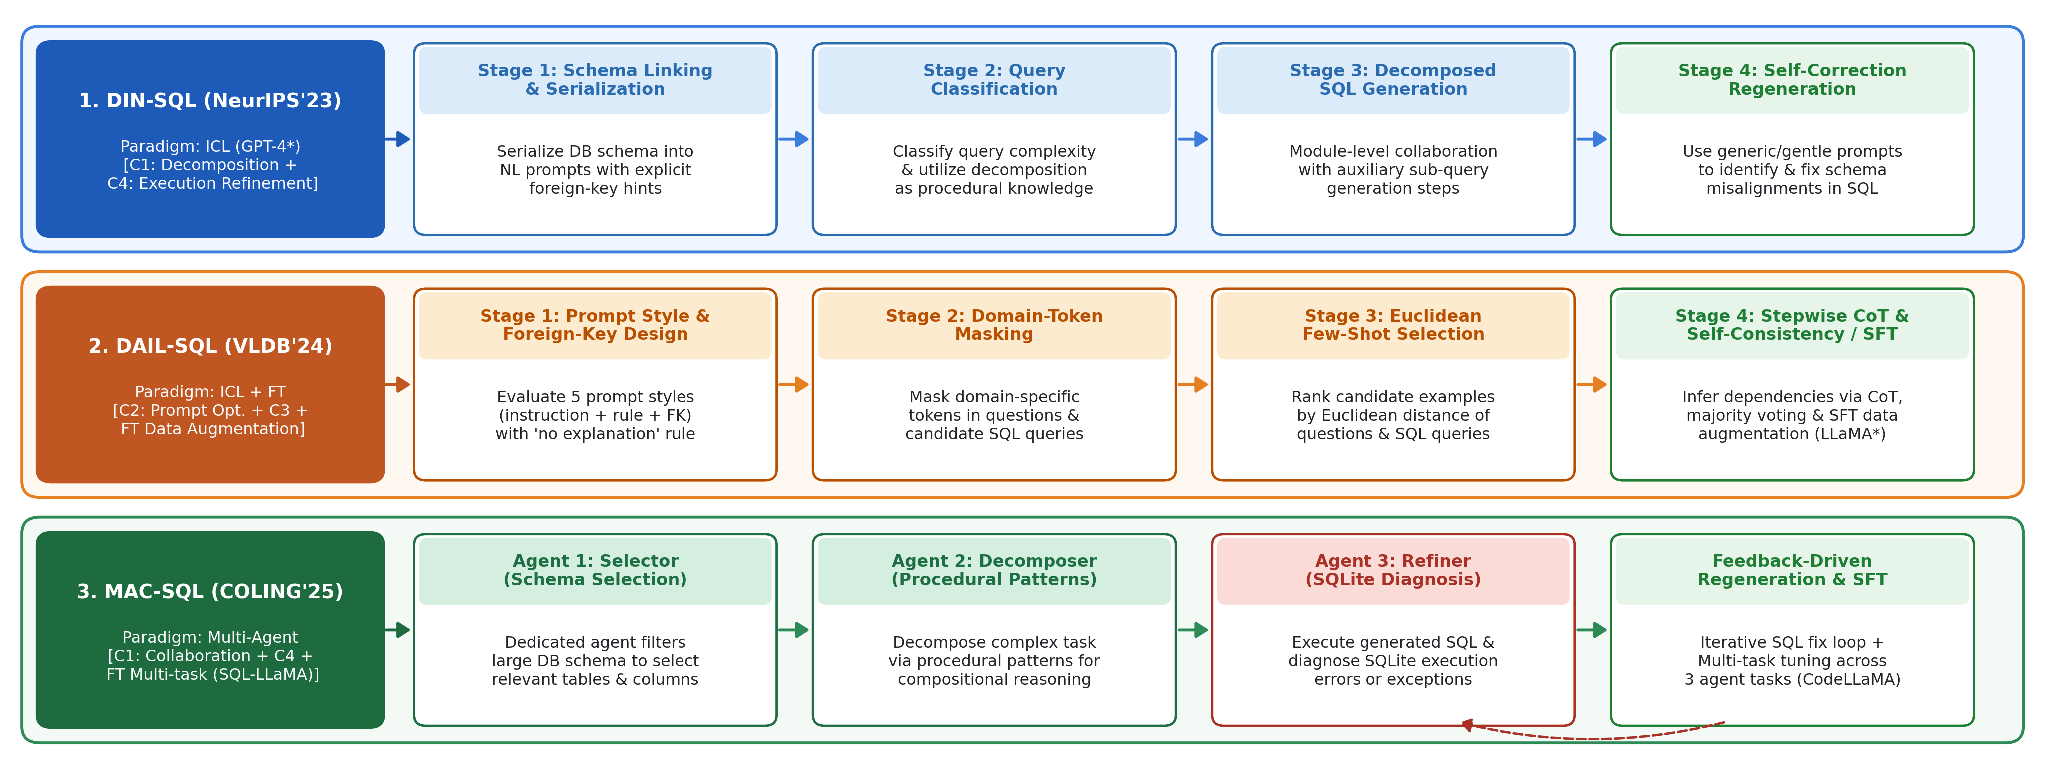
\includegraphics[width=0.95\linewidth,height=0.68\textheight,keepaspectratio]{04-method-architectures}
\caption{Kiến trúc DIN-SQL, DAIL-SQL, MAC-SQL \cite{ref1}}\label{fig:04-method-architectures}
\end{figure}

\section{So sánh tổng hợp các phương pháp tiêu biểu}

Bảng 3.1 trích đặc trưng các phương pháp tiêu biểu từ Bảng II, III, IV của \cite{ref1}.

\begingroup
\renewcommand{\arraystretch}{1.0}
\scriptsize
\setlength{\TableWidth}{\dimexpr\textwidth-24pt\relax}
\begin{longtable}{@{}>{\raggedright\arraybackslash}p{0.1400\TableWidth}@{\hspace{6pt}}>{\raggedright\arraybackslash}p{0.1000\TableWidth}@{\hspace{6pt}}>{\raggedright\arraybackslash}p{0.4300\TableWidth}@{\hspace{6pt}}>{\raggedright\arraybackslash}p{0.1300\TableWidth}@{\hspace{6pt}}>{\raggedright\arraybackslash}p{0.2000\TableWidth}@{}}
\caption{Đối sánh các phương pháp LLM-based Text-to-SQL tiêu biểu \cite{ref1}}\label{tab:report-2}\\
\toprule
\textbf{Phương pháp} & \textbf{Công bố} & \textbf{Phân loại \& cơ chế kỹ thuật cốt lõi (Bảng II, III, IV \cite{ref1})} & \textbf{LLM áp dụng} & \textbf{Bộ dữ liệu \& độ đo \cite{ref1}} \\
\midrule
\endfirsthead
\toprule
\textbf{Phương pháp} & \textbf{Công bố} & \textbf{Phân loại \& cơ chế kỹ thuật cốt lõi (Bảng II, III, IV \cite{ref1})} & \textbf{LLM áp dụng} & \textbf{Bộ dữ liệu \& độ đo \cite{ref1}} \\
\midrule
\endhead
\midrule
\endfoot
\bottomrule
\endlastfoot
\textbf{DIN-SQL \cite{ref4}} & NeurIPS'23 & ICL (C1 + C4): pipeline 4 bước (schema linking, classification, SQL generation, self-correction bằng gentle prompts). & GPT-4\textasteriskcentered{} & Spider, BIRD, Spider 2.0 (EX, EM, VES) \\
\textbf{C3 \cite{ref11}} & arXiv'23 & ICL (C1 + C2 + C4): ba mô-đun gồm schema linking bằng clear prompting, calibration bias prompting và consistency-based voting. & ChatGPT & Spider (EX) \\
\textbf{DAIL-SQL \cite{ref5}} & VLDB'24 & ICL (C2 + C3) \& FT (Data Aug.): 5 kiểu prompt, “no explanation”, mask token miền, Euclidean distance, self-consistency, SFT. & GPT-4\textasteriskcentered{}, LLaMA\textasteriskcentered{} & Spider, BIRD, Spider-Realistic, Spider 2.0 (EX, EM, VES) \\
\textbf{MAC-SQL \cite{ref6}} & COLING'25 & ICL (C1 + C4) \& FT (Multi-task): agent cho schema selection, decomposition, refinement (Refiner) \& SQL-LLaMA. & GPT-4\textasteriskcentered{}, CodeLLaMA & Spider, BIRD (EX, EM, VES) \\
\textbf{CodeS \cite{ref10}} & SIGMOD'24 & FT (Pre-training + Data Aug.): incremental pre-training ba giai đoạn; tăng cường dữ liệu bằng sinh hai chiều có ChatGPT hỗ trợ. & StarCoder & Spider, BIRD, Spider 2.0 (EX, VES) \\
\textbf{SuperSQL \cite{ref12}} & VLDB'24 & ICL (C1 + C2 + C3): hybrid integration giữa decomposition và prompt optimization; self-consistency bằng majority voting. & GPT-4\textasteriskcentered{} & Spider, BIRD (EX, EM, VES) \\
\textbf{CHASE-SQL \cite{ref13}} & ICLR'25 & ICL (C3 + C4): multi-path reasoning bằng “divide and conquer” CoT; agent Query Fixer chẩn đoán lỗi SQLite. & Gemini-1.5\textasteriskcentered{} & Spider, BIRD (EX, VES) \\
\textbf{ReFoRCE \cite{ref14}} & arXiv'25 & ICL (C1 + C2 + C3 + C4): table compression, column exploration cho schema dài; loại SQL chạy lỗi rồi voting. & o1-preview\textasteriskcentered{} & Spider 2.0 (EX) \\
\end{longtable}
\endgroup

Ở Mục V-B \cite{ref1}, nhóm tác giả rút ra ba nhận xét: (1) các loại ICL bổ trợ nhau vì mỗi loại có giới hạn riêng (Mục V-B1): C1 dễ lan truyền lỗi qua nhiều giai đoạn, C2 vướng giới hạn suy luận vốn có, C3 tăng mạnh chi phí tính toán, C4 phụ thuộc khả năng truy cập CSDL; (2) xu hướng gần đây là kết hợp nhiều loại (\emph{hybrid integration}), như SuperSQL \cite{ref12} gồm C1-C3 và ReFoRCE \cite{ref14} gồm cả C1-C4; (3) FT đánh đổi giữa chuyên biệt hóa và tổng quát hóa, có loại tốn tài nguyên, có loại dễ \emph{overfitting} (Mục V-B2), và nhiều khả năng cộng sinh (\emph{symbiotic}) với ICL: FT xây năng lực SQL nền, ICL thích ứng nhẹ không cần huấn luyện lại (Mục V-B3).

